\documentclass{beamer}
\usepackage[utf8]{inputenc}
\usepackage{uniinput}
\usepackage{proof}
\usepackage[english]{babel}
\usepackage{xstring}
\usepackage{ulem}
\usepackage{boxedminipage} 
\usepackage{xspace} 

\usepackage{tikz}
\usetikzlibrary{chains,fit,shapes}

\usetheme{Madrid}
\usecolortheme{seahorse}
\setbeamertemplate{navigation symbols}{}
\setbeamertemplate{footline}[frame number]
\setbeamertemplate{headline}{%
\leavevmode%
  \hbox{%
    \begin{beamercolorbox}[wd=\paperwidth,ht=2.5ex,dp=1.125ex]{palette quaternary}%
    \insertsectionnavigationhorizontal{\paperwidth}{}{\hskip0pt plus1filll}
    \end{beamercolorbox}%
  }
}

\newcommand{\SO}{\ensuremath{\mathrm{SO}}}
\newcommand{\FO}{\ensuremath{\mathrm{FO}}}
\newcommand{\NP}{{\rm NP}\xspace}
\newcommand{\SAT}{{\rm SAT}\xspace}
\newcommand{\structa}{\ensuremath{\mathfrak{A}}}
\newcommand{\minel}{\ensuremath{\underline{\mathrm{min}}}}
\newcommand{\blankcell}{\ensuremath{T_{\Box}}}
\newcommand{\nonblankcell}{\ensuremath{T_{\blacksquare}}}

\title{Turing Machines and Finite Models}
\author{Matthias Schlaipfer \and Sebastian Zivota}
\date{February 5, 2015}

\begin{document}

\begin{frame}[plain]
	\titlepage
\end{frame}

%\begin{frame}
%	\frametitle{Outline}
%	\tableofcontents
%\end{frame}

\begin{frame}
  \frametitle{Outlook}
  \begin{itemize}
    \item Connection between finite model theory and complexity theory
    \item By coding Turing machines in various logics
  \end{itemize}
  \vspace{2em} 
  \begin{alertblock}{Important Results}
  \begin{itemize}
    \item Trakhtenbrot's theorem: Finite satisfiability is undecidable
    \item Fagin's theorem: $\exists \SO$ captures $\mathrm{NP}$
  \end{itemize}
  \end{alertblock}
\end{frame}

\section{Background}

\begin{frame}
  \frametitle{Turing Machines}

  \begin{block}{Notation}
    $M = (Q, \Sigma, \Delta, \delta, q_0, Q_a, Q_r)$
    \begin{itemize}
      \item $Q$ \ldots states
      \item $\Sigma$ \ldots input alphabet
      \item $\Delta$ \ldots tape alphabet
      \item $\delta$ \ldots transition function
      \item $q_0$ \ldots initial state
      \item $Q_a$ / $Q_r$ \ldots accepting / rejecting states
    \end{itemize}

  \end{block}

  \begin{center}
  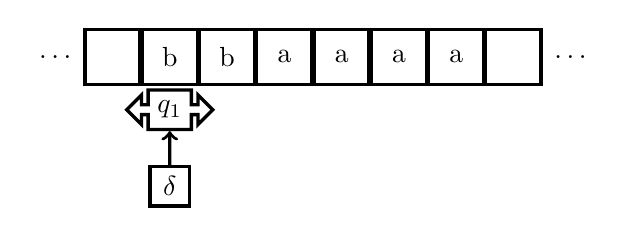
\begin{tikzpicture}
    \tikzstyle{every path}=[very thick]

    \edef\sizetape{0.7cm}
    \tikzstyle{tmtape}=[draw,minimum size=\sizetape]
    \tikzstyle{tmhead}=[arrow box,draw,minimum size=.5cm,arrow box
    arrows={east:.25cm, west:0.25cm}]
    \tikzstyle{tmprog}=[draw,minimum size=.5cm]

    %% Draw TM tape
    \begin{scope}[start chain=1 going right,node distance=-0.15mm]
        \node [on chain=1,tmtape,draw=none] {$\ldots$};
        \node [on chain=1,tmtape] {};
        \node [on chain=1,tmtape] (input) {b};
        \node [on chain=1,tmtape] {b};
        \node [on chain=1,tmtape] {a};
        \node [on chain=1,tmtape] {a};
        \node [on chain=1,tmtape] {a};
        \node [on chain=1,tmtape] {a};
        \node [on chain=1,tmtape] {};
        \node [on chain=1,tmtape,draw=none] {$\ldots$};
    \end{scope}

    %% Draw TM head below (input) tape cell
    \node [tmhead,yshift=-.3cm] at (input.south) (head) {$q_1$};
    \node [tmprog,yshift=-.7cm] at (head.south) (prog) {$\delta$};
    \draw [->] (prog) to (head);

    \end{tikzpicture}
    \nocite{tm_figure}
    \end{center}
  
\end{frame}

\begin{frame}
  \frametitle{Some Results on TM}

  \begin{itemize}
    \item The \textbf{halting problem} is undecidable.
    \item The \textbf{blank tape halting problem} is undecidable.
      \begin{center}
        \begin{boxedminipage}{.5\textwidth}
          \begin{tabbing}
            \quad\=\quad\=\quad\=\kill\\
                {\tt halts?}$(M,x)$\\
                \>{\tt if} $\mathsf{encode}(\mathsf{sim}(M, x)) \in \mathbf{BTHP}$\\
                \>\>yes\\
                \>{\tt else}\\
                \>\>no\\
          \end{tabbing}
        \end{boxedminipage}
      \end{center}
  \end{itemize}

  
\end{frame}

\begin{frame}
  \frametitle{Some Results on FOL}

  \begin{itemize}
    \item Completeness: a sentence $\phi$ is valid iff it is provable
    \item Proofs can be enumerated $\longrightarrow$ valid $\FO$ sentences
    recursively enumerable
  \end{itemize}

  \begin{definition}[Validity]
    All structures $\structa$, finite or infinite, are models of $\phi$.
    ($\structa \models \phi$)
  \end{definition}
  
\end{frame}

\section{Trakhtenbrot's Theorem}

\begin{frame}
  \frametitle{Trakhtenbrot's Theorem and Failure of Completeness}

  \begin{definition}[Finite satisfiability]
    Given a vocabulary $\sigma$, a sentence $\phi$ in that vocabulary is called
    finitely satisfiable if there is a finite structure $\structa \in
    \mathrm{STRUCT}[\sigma]$ such that $\structa \models \phi$.
  \end{definition}
  
  \pause

  \begin{theorem}[Trakhtenbrot]
    For every relational vocabulary $\sigma$ with at least one binary relation
    symbol, it is undecidable whether a sentence $\phi$ of vocabulary
    $\sigma$ is finitely satisfiable.
  \end{theorem}

\end{frame}

\begin{frame}
  \frametitle{Proof Idea}

  \begin{itemize}
    \item Code Turing machines in $\FO$
    \item For every TM $M$, construct a sentence $\phi_M$ of vocabulary $\sigma$
    such that $\phi_M$ is finitely satisfiable iff $M$ halts on the empty input.
  \end{itemize}

\end{frame}

\begin{frame}
  \frametitle{Definitions}

  \begin{itemize}
    \item $\sigma = \{<, \minel, \blankcell(\cdot, \cdot),
    \nonblankcell(\cdot,\cdot), (H_q(\cdot, \cdot))_{q \in Q}\}$\\
    \item $<$ is a linear order and $\minel$ is its minimal element (time,
    positions)
    \item Tape predicates $\blankcell(p,t), \nonblankcell(p,t)$
    \item Head predicates $H_q(p,t)$
  \end{itemize}
 
  
\end{frame}

\begin{frame}
  \frametitle{Definitions}

  For example at time $t$:
  \begin{center}
  \begin{tikzpicture}
    \tikzstyle{every path}=[very thick]

    \edef\sizetape{0.7cm}
    \tikzstyle{tmtape}=[draw,minimum size=\sizetape]
    \tikzstyle{tmhead}=[arrow box,draw,minimum size=.5cm,arrow box
    arrows={east:.25cm, west:0.25cm}]
    \tikzstyle{tmprog}=[draw,minimum size=.5cm]

    %% Draw TM tape
    \begin{scope}[start chain=1 going right,node distance=-0.15mm]
        \node [on chain=1,label={[label distance=2ex,text depth=5ex,rotate=90]right:$\minel$},tmtape] {$\Box$};
        \node [on chain=1,label={[label distance=2ex,text depth=5ex,rotate=90]right:$\minel+1$},tmtape] (input) {$\blacksquare$};
        \node [on chain=1,label={[label distance=2ex,text depth=5ex,rotate=90]right:$\minel+2$},tmtape] {$\blacksquare$};
        \node [on chain=1,label={[label distance=2ex,text depth=5ex,rotate=90]right:$\minel+3$},tmtape] (blankcell) {$\Box$};
        \node [on chain=1,label={[label distance=2ex,text depth=5ex,rotate=90]right:$\minel+4$},tmtape] {$\Box$};
        \node [on chain=1,label={[label distance=2ex,text depth=5ex,rotate=90]right:$\minel+5$},tmtape] {$\Box$};
        \node [on chain=1,label={[label distance=2ex,text depth=5ex,rotate=90]right:$\minel+6$},tmtape] {$\Box$};
        \node [on chain=1,label={[label distance=2ex,text depth=5ex,rotate=90]right:$\minel+7$},tmtape] {$\Box$};
        \node [on chain=1,tmtape,draw=none] {$\ldots$};
    \end{scope}

    %% Draw TM head below (input) tape cell
    \node [tmhead,yshift=-.3cm] at (input.south) (head) {$q_9$};
    %\node [tmprog,yshift=-1.7cm] at (head.south) (prog) {$\delta$};
    %\draw [->] (prog) to (head);

    \node at (4,-1) {$\blankcell(\minel+3, t)$} edge[->,bend left=15] (blankcell.south);
    \node at (3,-2) {$H_{q_9}(\minel+1, t)$} edge[->,bend left=25] (head.south);

    \end{tikzpicture}
    \nocite{tm_figure}
    \end{center}
  
\end{frame}

\begin{frame}
  \frametitle{Encoding}

  \centering
  \begin{enumerate}
    \only<1->{\item $<$ is a linear order and $\minel$ is its minimal element}
    \only<2->{\item Initially the tape is blank}
      \only<2>{\begin{align*}
        H_{q_0}(\minel, \minel) \wedge \forall p \; \blankcell(p, \minel)
      \end{align*}}
    \only<3->{\item Either a cell is blank or not}
      \only<3>{\begin{align*}
        \forall p \forall t \;
        \left(\blankcell(p, t)
        \Leftrightarrow \neg \nonblankcell(p, t)\right)
      \end{align*}}
    \only<4->{\item Machine is in one state at a time}
      \only<4>{\begin{align*}
        \forall t \exists !p &\left( \bigvee_{q \in Q} H_q(p,t) \right)
        \wedge \\ \neg \exists p \exists t &\left( \bigvee_{q, q' \in Q, q \neq q'}
        H_q(p, t) \wedge H_{q'}(p,t) \right)
      \end{align*}}
    \only<5->{\item Machine respects the transition relation}\only<5>{ e.g.
    $\delta(q, \Box) = (q', \blacksquare, \ell)$}
      \only<5>{\small \begin{align*}
        \forall p \forall t \;
        \left(
          \begin{array}{cc}
                   & p \neq \minel\\
            \wedge & \blankcell(p, t)\\
            \wedge & H_q(p,t)
          \end{array}
        \right)
          \Rightarrow
        \left(
          \begin{array}{cl}
                   & \nonblankcell(p, t+1)\\
            \wedge & H_{q'}(p-1, t+1)\\
            \wedge &
              \begin{array}[x]{@{}l@{}} 
            \forall p' \; \left(p \neq p' \Rightarrow \right. \\ \left. \left( \bigwedge_{i =
            \Box,\blacksquare} T_i(p',t+1) \Leftrightarrow
            T_i(p',t)\right)\right)
              \end{array}
          \end{array}
        \right)
      \end{align*}}
    \only<6->{\item Finally, the machine halts}
      \only<6>{\begin{align*}
        \exists p \exists t \; \bigvee_{q \in Q_a \cup Q_r} H_q(p,t)
      \end{align*}}
  \end{enumerate}
  
\end{frame}

\begin{frame}
  \frametitle{Proof}

  \begin{theorem}[Trakhtenbrot]
    For every relational vocabulary $\sigma$ with at least one binary relation
    symbol, it is undecidable whether a sentence $\phi$ of vocabulary
    $\sigma$ is finitely satisfiable.
  \end{theorem}
  
  \begin{alertblock}{Proof}

  \begin{itemize}
    \item A finite model of $\phi_M$ represents a computation of $M$ starting
    from blank tape to a halting state
    \item The set of all configurations of the halting computations of $M$ is a
    finite model of $\phi_M$
  \end{itemize}

  $M$ halts on the empty input iff $\phi_M$ has a finite model. Since
  \textbf{BTHP} is undecidable, so is finite satisfiability for $\phi_M$.
  \end{alertblock}
  
\end{frame}

\begin{frame}
  \frametitle{Corollaries}

  \begin{corollary}[Failure of completeness in the finite]
    For any vocabulary containing at least one binary relation symbol, the set
    of finitely valid sentences is not recursively enumerable.
  \end{corollary}

  \begin{corollary}[No analog to Löwenheim-Skolem for finite models]
    There is no recursive function $f$ such that if $\phi$ has a finite model,
    then it has a model of size at most $f(\phi)$.
  \end{corollary}
  
\end{frame}

\begin{frame}
  \frametitle{Corollaries}

  \begin{corollary}[Cook]
    \SAT is \NP-complete
  \end{corollary}

  \begin{alertblock}{Proof}
    $\mathcal{P} \in \NP$
    \begin{itemize}
      \item $\phi \equiv \exists S_1, \ldots, \exists S_n \; \varphi$, such that
      $\structa$ is in $\mathcal{P}$ iff $\structa \models \phi$ (Fagin)
      \item $X = \{S_i(\vec{a}) \; | \; i = 1, \ldots, n, \vec{a} \in
      A^{\text{arity}(S_i)}\}$
      \item $\structa \models \phi$ iff $\alpha_{\phi}^{\structa}$ is
      satisfiable
      \item $\alpha_{\varphi}^{\structa}$ is obtained from $\varphi$
        \begin{itemize}
          \item replace $\exists x \, \psi(x, \cdot)$ by $\bigvee_{a \in A}
          \psi(a, \cdot)$
          \item replace $\forall x \, \psi(x, \cdot)$ by $\bigwedge_{a \in A}
          \psi(a, \cdot)$
          \item replace $R(\vec{a})$, for $R \in \sigma$ by its truth value in
          $\structa$
        \end{itemize}
      \item $\structa \models \phi$ iff $\alpha_{\varphi}^{\structa}$ is
      satisfiable. $\alpha_{\varphi}^{\structa}$ can be constructed by
      deterministic logarithmic space machine
    \end{itemize}
  \end{alertblock}
  
\end{frame}

\section{}
\bibliography{presentation}
\bibliographystyle{plain}

\end{document}
